\documentclass[12pt,a4paper,danish]{article}

\usepackage[danish]{babel}
\usepackage[utf8]{inputenc}
\usepackage[T1]{fontenc}
\usepackage{graphicx}

\begin{document}
\title{Gruppeøvelse 2}
\author{Anders Kiel Hovgaard\\Rúni Klein Hansen}
\date{20 oktober 2013}
\maketitle

\section{Introduktion}
En pipelined MIPS implementation, baseret på figur 4.60 s. 375 COD.
Disse instruktioner virker:
\begin{itemize}
  \item addu, addiu
  \item slt, slti
  \item subu
  \item and, andi
  \item or, ori
  \item lw
\end{itemize}

Disse kommandoer virker ikke:
\begin{itemize}
  \item sw
  \item beq*
  \item jal*
  \item jr*
\end{itemize}
*Disse instruktioner skal have support for et branch delay slot.\\

Vi har prøvet at implementere forwarding, men har fået det til at fungere endnu, 
så der forekommer data hazards. Vores stalling ikke fungerer, så 
der bliver ikke indsat nop instruktioner og da forwarding ikke virker, vil der ikke 
blive sent opdaterede resultater til næste instruktion. Denne begrænsing, pipelining 
uden forwarding og stalling giver hurtigt problemer, fx. ville denne kombination 
af instruktioner:
\begin{verbatim}
  addiu $t0, $t0, 5
  addiu $t1, $t0, 5
\end{verbatim}
give samme resultat, \textbf{\$t0 = \$t1}, da \textbf{\$t0} først bliver 5, tre 
clock cycler senere. 

Der er ikke support for jumps, så beq, jal og jr virker ikke.
\section{Overview}
\begin{figure}[h!]
\centering
  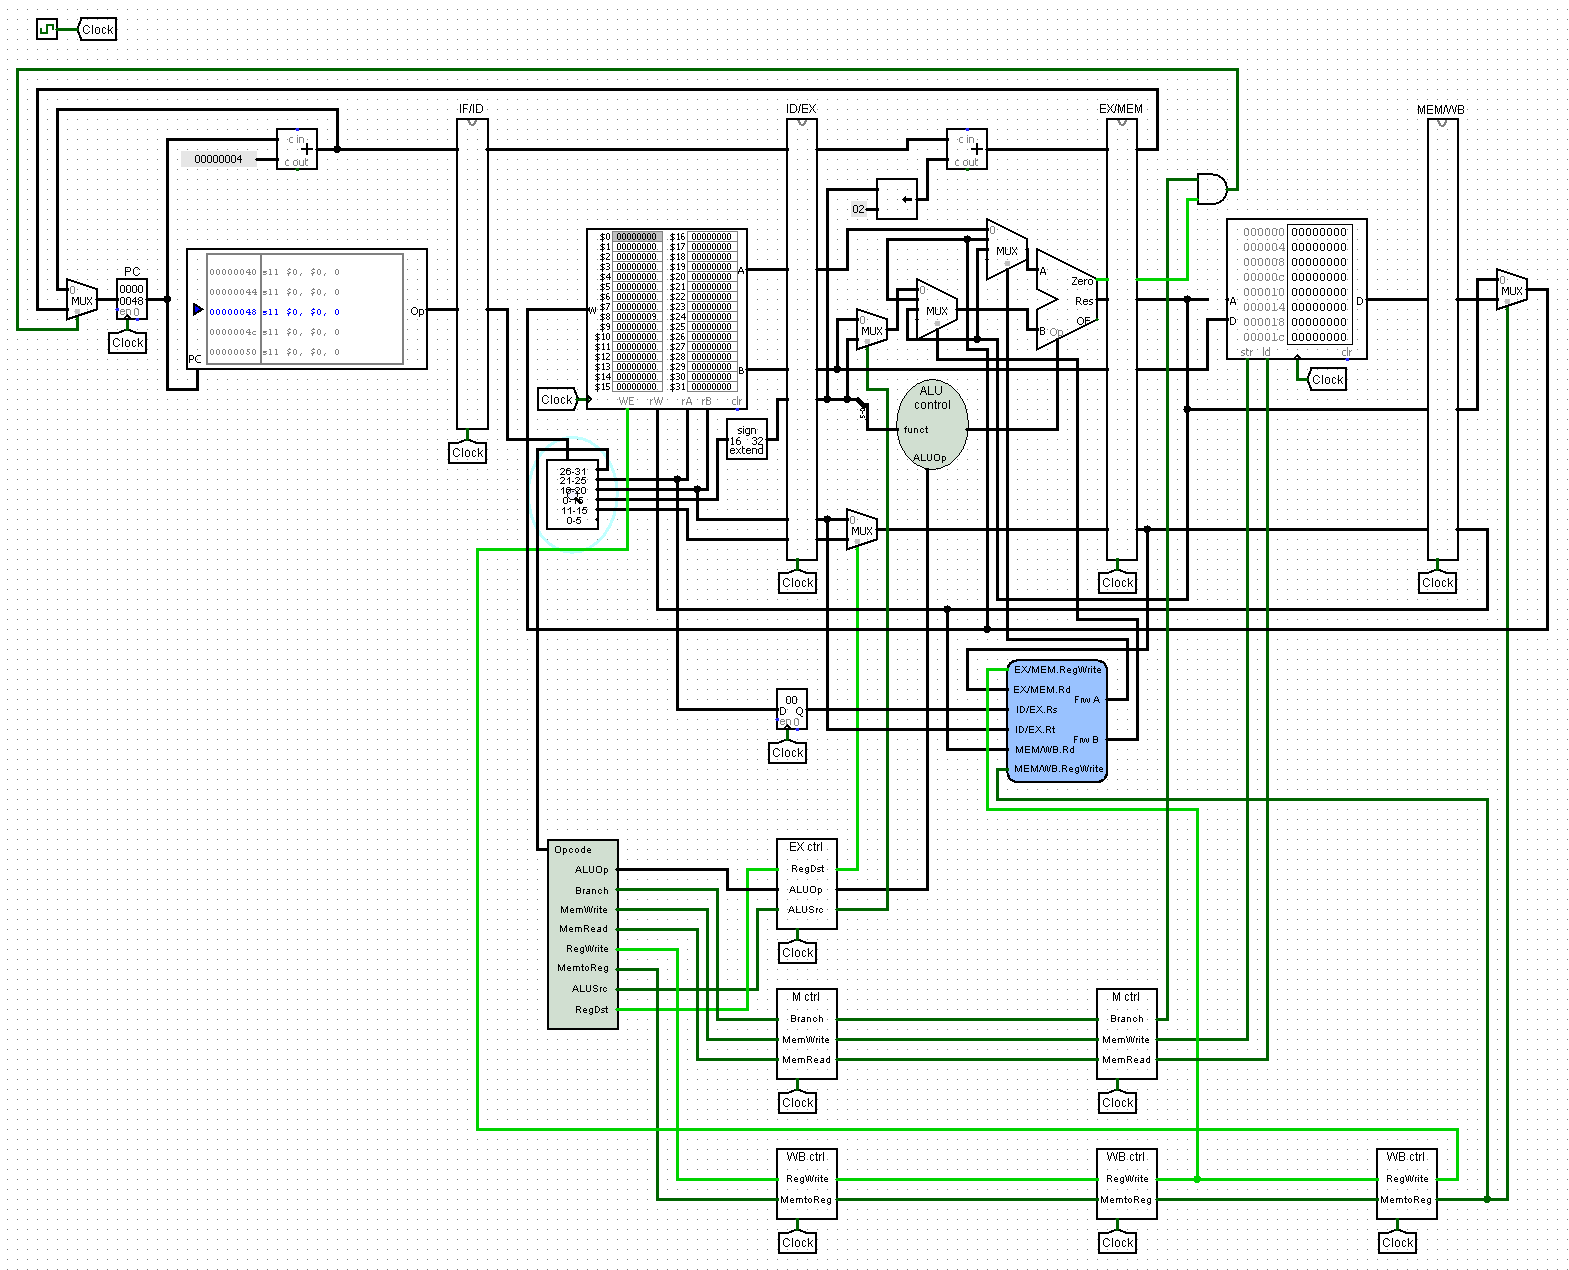
\includegraphics[scale=0.4]{circuit.png}
  \caption{Kredsøb af MIPS implementation med pipelining}
  \label{fig:mips}
\end{figure}
Pipelinet er opdelt i fem "stages": IF(Instruction fetch), ID(Instruction decode/register file 
read), EX(Execution/Address calculation), MEM(Memory access) og WB(Write-back).



\end{document}
